% White paper for the nonparax package. Compile with: latexmk -pdf nonparax.tex
\documentclass[
	aps,
	pra,
	reprint,
	amsmath,
	amssymb,
	superscriptaddress,
	nofootinbib
]{revtex4-2}

\usepackage{booktabs}
\usepackage[dvipsnames]{xcolor}
\usepackage{tikz}
\usetikzlibrary{arrows.meta,calc,decorations.markings,decorations.pathreplacing}
\usepackage{tikz-3dplot}
\usepackage{microtype}
\usepackage[colorlinks=true,citecolor=blue,linkcolor=blue,urlcolor=blue]{hyperref}
\usepackage{xurl}

\definecolor{capl}{HTML}{0072B2}    % aplanatic lens
\definecolor{cthin}{HTML}{D55E00}   % thin lens
\definecolor{cspec}{HTML}{009E73}   % Gaussian spectrum

\newcommand{\affilANU}{Research School of Physics, Australian National University, Canberra ACT 2601, Australia}

\begin{document}

\title{Gaussian Beams Beyond the Paraxial Approximation}

\author{Ivan Toftul}
\affiliation{\affilANU}
\author{Claude Code}
\noaffiliation

\date{\today}

\begin{abstract}
Beyond the paraxial limit the name ``Gaussian beam'' does not define a unique field. One must say where the Gaussian is: in the angular spectrum, or in the pupil of a lens. We write six such beams as exact solutions of Maxwell's equations, each fixed by an envelope $a(\theta)$ and a polarization rule $c(\theta)$. They include the beams of COMSOL and of the Optical Tweezers Toolbox.
\end{abstract}

\maketitle

% =====================================================================
\section{Paraxial Gaussian beam}

The time dependence is $e^{-i\omega t}$, and the units are SI. The medium is homogeneous and lossless, with the absolute permittivity $\varepsilon$, the absolute permeability $\mu$, the index $n=c\sqrt{\varepsilon\mu}$ and the wavenumber $k=\omega\sqrt{\varepsilon\mu}=2\pi n/\lambda$. The position is $\mathbf r=(\rho,\varphi,z)$ in cylindrical coordinates.

The paraxial Gaussian beam reads~\cite{Novotny2012}
\begin{align}
\begin{split}
    \sqrt{\varepsilon}\mathbf{E} &= \mathcal{A}_0 \: \mathbf{u} \frac{w_0}{w(z)} e^{- \frac{\rho^2}{w^2(z)}} e^{i \left[ k z - \eta(z) + R^{-1}(z) k \rho^2 / 2 \right]}, \\
    \sqrt{\mu}\mathbf{H} &= \mathbf{\hat{z}} \times \sqrt{\varepsilon}\mathbf{E},
\end{split}
\label{eq:paraxial}
\end{align}
where $\mathcal{A}_0 / \sqrt{\varepsilon}$ is the electric field amplitude, $\mathbf{u}$ is the unit complex polarization vector, $w(z) = w_0 \sqrt{1 + z^2/z_0^2}$ is the beam radius, $R^{-1}(z) = z/(z^2 + z_0^2)$ is the inverse wavefront radius, $\eta(z) = \arctan(z/z_0)$ is the Gouy phase, and $z_0 = k w_0^2 / 2$ is the Rayleigh range. We use the circular polarization vectors
\begin{equation}
    \mathbf{\hat{e}}_\sigma=(\mathbf{\hat{x}}+i \sigma\mathbf{\hat{y}})/\sqrt{2},
    \label{eq:esigma}
\end{equation}
with the handedness $\sigma=\pm1$.

Equation~\eqref{eq:paraxial} solves the paraxial wave equation, not Maxwell's equations, and it needs $kw_0\gg2$. Beyond this limit no closed-form Gaussian beam exists, and the name ``Gaussian beam'' no longer defines a unique field. One must say where the Gaussian is. It can be in the angular spectrum, in the pupil of an aplanatic lens, or in the pupil of a thin lens. The code for all beams below is in Ref.~\cite{toftul2026github_nonparax}.

\begin{figure}[t]
\centering
\tdplotsetmaincoords{65}{115}
\begin{tikzpicture}[tdplot_main_coords, >=Latex, font=\footnotesize, scale=1.6,
                    baseline=(current bounding box.north)]
  \def\th{40}\def\ph{55}
  \pgfmathsetmacro{\ct}{cos(\th)}\pgfmathsetmacro{\st}{sin(\th)}
  \pgfmathsetmacro{\cp}{cos(\ph)}\pgfmathsetmacro{\sp}{sin(\ph)}
  \coordinate (O) at (0,0,0);
  \coordinate (K) at ({\st*\cp},{\st*\sp},{\ct});
  \coordinate (Kxy) at ({\st*\cp},{\st*\sp},0);
  \draw[->] (O) -- (1.25,0,0) node[anchor=north east] {$x$};
  \draw[->] (O) -- (0,1.25,0) node[anchor=north west] {$y$};
  \draw[->] (O) -- (0,0,1.3) node[anchor=south] {$z$};
  \draw[dotted] plot[domain=-10:100,samples=40] ({cos(\x)},{sin(\x)},0);
  \draw[dotted] plot[domain=0:95,samples=40] ({sin(\x)*\cp},{sin(\x)*\sp},{cos(\x)});
  \fill[cspec,opacity=0.12] (O) -- (0,0,1) -- plot[domain=0:\th,samples=20] ({sin(\x)*\cp},{sin(\x)*\sp},{cos(\x)}) -- cycle;
  \draw[->,very thick] (O) -- (K) node[anchor=south east] {$\mathbf{\hat{k}}$};
  \draw[dashed] (K) -- (Kxy) (O) -- (Kxy);
  \draw[->,capl] plot[domain=0:\ph,samples=20] ({0.35*cos(\x)},{0.35*sin(\x)},0);
  \node[capl] at ({0.48*cos(\ph/2)},{0.48*sin(\ph/2)},0) {$\phi$};
  \draw[->,capl] plot[domain=0:\th,samples=20] ({0.45*sin(\x)*\cp},{0.45*sin(\x)*\sp},{0.45*cos(\x)});
  \node[capl] at ({0.58*sin(\th/2)*\cp},{0.58*sin(\th/2)*\sp},{0.58*cos(\th/2)}) {$\theta$};
  \draw[->,thick,cthin] (K) -- ++({0.4*\ct*\cp},{0.4*\ct*\sp},{-0.4*\st}) node[anchor=west] {$\mathbf{\hat{\boldsymbol{\theta}}}$};
  \draw[->,thick,cthin] (K) -- ++({-0.4*\sp},{0.4*\cp},0) node[anchor=west] {$\mathbf{\hat{\boldsymbol{\phi}}}$};
  \fill (O) circle (0.6pt);
  \node[anchor=north west, inner sep=0pt, font=\sffamily\bfseries\small]
    at (current bounding box.north west) {A};
\end{tikzpicture}%
\hspace{0.8em}%
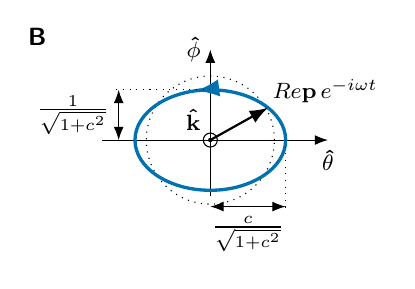
\begin{tikzpicture}[>=Latex, font=\footnotesize, scale=1.15,
                    baseline=(current bounding box.north)]
  \def\c{1.5}\def\wt{40}
  \pgfmathsetmacro{\u}{\c/sqrt(1+\c*\c)}\pgfmathsetmacro{\v}{1/sqrt(1+\c*\c)}
  \draw[->] (-1.2,0) -- (1.3,0) node[below] {$\mathbf{\hat{\boldsymbol{\theta}}}$};
  \draw[->] (0,-0.62) -- (0,1.0) node[left] {$\mathbf{\hat{\boldsymbol{\phi}}}$};
  \draw[dotted] (0,0) circle ({1/sqrt(2)});
  \draw[very thick,capl] (0,0) ellipse ({\u} and {\v});
  \draw[->,very thick,capl] (100:{\u} and {\v}) -- (101:{\u} and {\v});
  \draw[->,thick] (0,0) -- ({\u*cos(\wt)},{\v*sin(\wt)}) node[above right=-2pt] {$\operatorname{Re}\mathbf p\,e^{-i\omega t}$};
  \draw[dotted] (\u,0) -- (\u,{-\v-0.25}) (0,\v) -- ({-\u-0.25},\v);
  \draw[<->] (0,{-\v-0.18}) -- (\u,{-\v-0.18}) node[below,pos=0.5] {$\frac{c}{\sqrt{1+c^2}}$};
  \draw[<->] ({-\u-0.18},0) -- ({-\u-0.18},\v) node[left,pos=0.5] {$\frac{1}{\sqrt{1+c^2}}$};
  \draw (0,0) circle (2.2pt); \fill (0,0) circle (0.7pt);
  \node[above left] at (0,0) {$\mathbf{\hat{{k}}}$};
  \node[anchor=north west, inner sep=0pt, font=\sffamily\bfseries\small]
    at (current bounding box.north west) {B};
\end{tikzpicture}
\caption{\textsf{\textbf{A}}~Angles and unit vectors of Eqs.~\eqref{eq:debye}--\eqref{eq:rule}. A plane wave travels along $\mathbf{\hat{k}}$; the meridional plane (shaded) holds $z$ and $\mathbf{\hat{k}}$.
\textsf{\textbf{B}}~The unit polarization vector $\mathbf p$ of one plane wave, Eq.~\eqref{eq:rule}, for $\sigma=+1$, viewed with $\mathbf{\hat k}$ out of the page. In time, $\operatorname{Re}\mathbf p\,e^{-i\omega t}$ traces an ellipse (blue) with the semi-axes $c/\sqrt{1+c^2}$ along $\mathbf{\hat{\boldsymbol{\theta}}}$ and $1/\sqrt{1+c^2}$ along $\mathbf{\hat{\boldsymbol{\phi}}}$, here $c=1.5$. For $c=1$ it is the dotted circle.}
\label{fig:angles_and_polarization}
\end{figure}

\begin{figure*}[t]
\centering
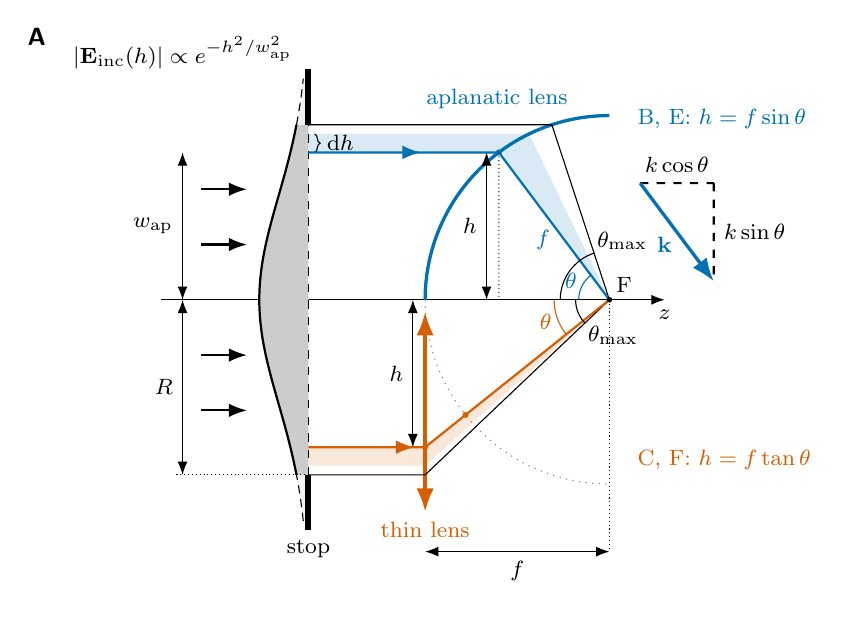
\begin{tikzpicture}[>=Latex, font=\footnotesize, scale=0.78, baseline=(current bounding box.north),
    ray/.style={thick, postaction={decorate},
      decoration={markings, mark=at position 0.3 with {\arrow{>}}}},
    dim/.style={<->, thin}]
  \def\f{3.0}      % focal length = radius of the reference sphere
  \def\xp{-4.9}    % pupil plane
  \def\h{2.4}      % drawn ray height, h = w_ap = 0.8 f  (k w0 = 2.5)
  \def\dh{0.3}     % width of the ray tube
  \def\R{2.85}     % stop radius, R = 0.95 f
  \def\Lk{2.0}     % drawn length of k
  \pgfmathsetmacro{\thB}{asin(\h/\f)}
  \pgfmathsetmacro{\thBb}{asin((\h+\dh)/\f)}
  \pgfmathsetmacro{\thC}{atan(\h/\f)}
  \pgfmathsetmacro{\zB}{-\f*cos(\thB)}
  \pgfmathsetmacro{\zBb}{-\f*cos(\thBb)}
  \pgfmathsetmacro{\thmB}{asin(\R/\f)}
  \pgfmathsetmacro{\thmC}{atan(\R/\f)}
  \coordinate (F) at (0,0);
  \coordinate (P) at (\zB,\h);
  \coordinate (L) at (-\f,-\h);
  % ray tubes [h, h+dh]: the same pupil strip goes into different solid angles
  \fill[capl,opacity=0.15] (\xp,\h) -- (P) -- (F) -- (\zBb,\h+\dh) -- (\xp,\h+\dh) -- cycle;
  \fill[cthin,opacity=0.15] (\xp,-\h) -- (L) -- (F) -- (-\f,-\h-\dh) -- (\xp,-\h-\dh) -- cycle;
  % optical axis
  \draw[->] (\xp-2.4,0) -- (0.9,0) node[below] {$z$};
  % pupil field |E_inc(h)| = e^{-h^2/w_ap^2}: passed by the stop (dark) and blocked (light)
  \fill[gray!10] plot[domain=-3.6:3.6,samples=100] ({\xp-0.8*exp(-(\x/\h)^2)},\x) -- (\xp,3.6) -- (\xp,-3.6) -- cycle;
  \fill[gray!40] plot[domain=-\R:\R,samples=100] ({\xp-0.8*exp(-(\x/\h)^2)},\x) -- (\xp,\R) -- (\xp,-\R) -- cycle;
  \draw[thick] plot[domain=-\R:\R,samples=100] ({\xp-0.8*exp(-(\x/\h)^2)},\x);
  \draw[thin,densely dashed] plot[domain=\R:3.6,samples=20] ({\xp-0.8*exp(-(\x/\h)^2)},\x)
                             plot[domain=-3.6:-\R,samples=20] ({\xp-0.8*exp(-(\x/\h)^2)},\x);
  \draw[dashed] (\xp,-\R) -- (\xp,\R);
  % aperture stop of radius R
  \draw[line width=2.2pt] (\xp,\R) -- (\xp,3.75) (\xp,-\R) -- (\xp,-3.75);
  \node[below] at (\xp,-3.75) {stop};
  \node[anchor=south east] at (\xp-0.1,3.6) {$|\mathbf E_\mathrm{inc}(h)|\propto e^{-h^2/w_\mathrm{ap}^2}$};
  \draw[dim] (\xp-2.05,0) -- (\xp-2.05,\h) node[pos=0.5,left] {$w_\mathrm{ap}$};
  \draw[dim] (\xp-2.05,0) -- (\xp-2.05,-\R) node[pos=0.5,left] {$R$};
  \draw[densely dotted] (\xp-2.15,-\R) -- (\xp,-\R);
  % the input beam travels along +z towards the lens
  \foreach \y in {-1.8,-0.9,0.9,1.8}
    \draw[->,thick] (\xp-1.75,\y) -- (\xp-1.0,\y);
  \draw[decorate,decoration={brace,amplitude=2pt}] (\xp+0.1,\h+\dh) -- (\xp+0.1,\h)
    node[pos=0.5,right=1pt] {$\mathrm{d}h$};
  % ---------------- upper half: aplanatic lens, h = f sin(theta)
  \draw[capl,very thick] (90:\f) arc (90:180:\f);
  \node[capl,anchor=south east] at (100:\f) {aplanatic lens};
  \draw (\xp,\R) -- ({180-\thmB}:\f) -- (F);                 % marginal ray
  \draw[ray,capl] (\xp,\h) -- (P) -- (F);
  \fill[capl] (P) circle (1.4pt);
  \path (P) -- (F) node[capl,pos=0.5,below left=-2pt] {$f$};
  \draw[densely dotted] (P) -- (\zB,0);
  \draw[dim] ({\zB-0.2},0) -- ({\zB-0.2},\h) node[pos=0.5,left] {$h$};
  \draw[capl] (180:0.5) arc (180:{180-\thB}:0.5);
  \node[capl] at ({180-\thB/2}:0.7) {$\theta$};
  \draw (180:0.8) arc (180:{180-\thmB}:0.8);
  \node[anchor=south west,inner sep=1pt] at ({180-\thmB}:0.8) {$\theta_{\max}$};
  % wavevector of the refracted ray (parallel to it): k sin(theta) / k = h / f
  \coordinate (S) at (0.5,1.9);
  \coordinate (Sh) at ($(S)+({\Lk*cos(\thB)},0)$);
  \coordinate (St) at ($(Sh)+(0,{-\Lk*sin(\thB)})$);
  \draw[dashed,thick] (S) -- (Sh) node[pos=0.5,above] {$k\cos\theta$};
  \draw[dashed,thick] (Sh) -- (St) node[pos=0.5,right] {$k\sin\theta$};
  \draw[->,very thick,capl] (S) -- (St) node[pos=0.5,below left=-2pt] {$\mathbf k$};
  % ---------------- lower half: thin lens, h = f tan(theta)
  \draw[gray,dotted] (180:\f) arc (180:270:\f);
  \draw[cthin,line width=1.2pt,<->] (-\f,-0.2) -- (-\f,-3.45) node[below] {thin lens};
  \draw (\xp,-\R) -- (-\f,-\R) -- (F);                       % marginal ray
  \draw[ray,cthin] (\xp,-\h) -- (L) -- (F);
  \fill[cthin] (L) circle (1.4pt);
  \fill[cthin] ({180+\thC}:\f) circle (1.4pt);
  \draw[dim] ({-\f-0.2},0) -- ({-\f-0.2},-\h) node[pos=0.5,left] {$h$};
  \draw[cthin] (180:0.9) arc (180:{180+\thC}:0.9);
  \node[cthin] at ({180+\thC/2}:1.1) {$\theta$};
  \draw (180:0.55) arc (180:{180+\thmC}:0.55);
  \node[anchor=north west,inner sep=1pt] at ({180+\thmC}:0.55) {$\theta_{\max}$};
  \draw[dim] (-\f,-4.1) -- (F|-0,-4.1) node[pos=0.5,below] {$f$};
  \draw[densely dotted] (F) -- (0,-4.1);
  \fill (F) circle (1.3pt) node[above right=-1pt] {F};
  % mappings
  \node[capl,anchor=west] at (0.3,2.95) {B, E: $h=f\sin\theta$};
  \node[cthin,anchor=west] at (0.3,-2.6) {C, F: $h=f\tan\theta$};
  \node[anchor=north west,inner sep=0pt,font=\sffamily\bfseries\small]
    at ($(current bounding box.north west)+(-0.6,0)$) {A};
\end{tikzpicture}%
\hspace{2em}%
% ------------------------------------------------ B: no lens, Gaussian angular spectrum (rules A, D)
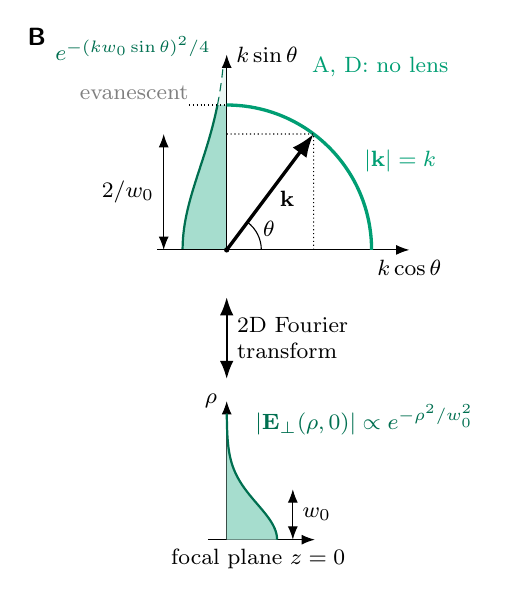
\begin{tikzpicture}[>=Latex, font=\footnotesize, scale=0.8, baseline=(current bounding box.north),
                    dim/.style={<->, thin}]
  \def\k{2.3}      % radius of the circle |k| = k
  \def\kb{1.84}    % 1/e point of the spectrum, 2/w0 = 0.8 k  (k w0 = 2.5)
  \def\wz{0.8}     % drawn w0 in the focal plane (real space, own scale)
  \def\yr{-4.6}    % base line of the real-space profile
  \pgfmathsetmacro{\th}{asin(\kb/\k)}
  \pgfmathsetmacro{\ct}{cos(\th)}
  \coordinate (O) at (0,0);
  \coordinate (P) at ({\k*\ct},\kb);
  % spectrum e^{-(w0 k sin(theta))^2/4}: propagating (dark) and evanescent (light)
  \fill[cspec!8] plot[domain=0:2.9,samples=80] ({-0.7*exp(-(\x/\kb)^2)},\x) -- (0,2.9) -- (0,0) -- cycle;
  \fill[cspec!35] plot[domain=0:\k,samples=80] ({-0.7*exp(-(\x/\kb)^2)},\x) -- (0,\k) -- (0,0) -- cycle;
  \draw[thick,cspec!70!black] plot[domain=0:\k,samples=80] ({-0.7*exp(-(\x/\kb)^2)},\x);
  \draw[thin,densely dashed,cspec!70!black] plot[domain=\k:2.9,samples=20] ({-0.7*exp(-(\x/\kb)^2)},\x);
  \node[cspec!70!black,anchor=south east] at (-0.1,2.85) {$e^{-(kw_0\sin\theta)^2/4}$};
  % axes
  \draw[->] (-1.1,0) -- (2.9,0) node[below] {$k\cos\theta$};
  \draw[->] (0,0) -- (0,3.1) node[right] {$k\sin\theta$};
  % propagating plane waves: |k| = k
  \draw[cspec,very thick] (0:\k) arc (0:90:\k);
  \node[cspec,anchor=south west] at (28:\k) {$|\mathbf k|=k$};
  \draw[densely dotted] (-0.6,\k) -- (0,\k);
  \node[gray,anchor=east] at (-0.45,2.5) {evanescent};
  \draw[dim] (-1.0,0) -- (-1.0,\kb) node[pos=0.5,left] {$2/w_0$};
  % one plane wave
  \draw[densely dotted] (0,\kb) -- (P) -- ({\k*\ct},0);
  \draw[->,very thick] (O) -- (P) node[pos=0.55,below right=-2pt] {$\mathbf k$};
  \draw (0.55,0) arc (0:\th:0.55); \node at ({\th/2}:0.75) {$\theta$};
  \fill (O) circle (1.2pt);
  \node[cspec,anchor=south west] at (1.2,2.6) {A, D: no lens};
  % focal plane: transverse field, the Fourier pair of the spectrum
  \draw[<->,thick] (0,-0.75) -- (0,-2.05) node[pos=0.5,right,align=left] {2D Fourier\\transform};
  \draw[->] (-0.3,\yr) -- (1.4,\yr);
  \draw[->] (0,\yr) -- (0,{\yr+2.2}) node[left] {$\rho$};
  \fill[cspec!35] plot[domain=0:2.0,samples=60] ({0.8*exp(-(\x/\wz)^2)},{\yr+\x}) -- (0,{\yr+2.0}) -- (0,\yr) -- cycle;
  \draw[thick,cspec!70!black] plot[domain=0:2.0,samples=60] ({0.8*exp(-(\x/\wz)^2)},{\yr+\x});
  \draw[dim] (1.05,\yr) -- (1.05,{\yr+\wz}) node[pos=0.5,right] {$w_0$};
  \node[below] at (0.5,\yr) {focal plane $z=0$};
  \node[cspec!70!black,anchor=west] at (0.3,{\yr+1.9}) {$|\mathbf E_\perp(\rho,0)|\propto e^{-\rho^2/w_0^2}$};
  \node[anchor=north west,inner sep=0pt,font=\sffamily\bfseries\small]
    at ($(current bounding box.north west)+(-0.3,0)$) {B};
\end{tikzpicture}
\caption{Where the Gaussian of each beam in Table~\ref{tab:env} lies, for $kw_0=2.5$.
\textsf{\textbf{A}}~Beams B, C, E, F. The input field~\eqref{eq:Einc} is bent towards the focus F by an aplanatic lens, $h=f\sin\theta$ (upper half), or by a thin lens, $h=f\tan\theta$ (lower half). The drawn rays are at $h=w_\mathrm{ap}$, which is the $1/e$ angle $\theta_b$ of beams E and F. The shaded tubes carry the power of the same strip $\mathrm{d}h$, which gives the prefactor in Eq.~\eqref{eq:lens}; E and F omit it. A stop of radius $R$ blocks $|h|>R$ and sets $\theta_{\max}$, with $\mathrm{NA}=n\sin\theta_{\max}$.
\textsf{\textbf{B}}~Beams A, D. The focal-plane field $e^{-\rho^2/w_0^2}$ (bottom) has the spectrum $e^{-(kw_0\sin\theta)^2/4}$ over the transverse wavevector $k\sin\theta$ (top), the same function of $\theta$ as for the aplanatic lens. The part $k\sin\theta>k$ is evanescent and not in Eq.~\eqref{eq:debye}.}
\label{fig:constructions}
\end{figure*}

\begin{table*}[t]
    \caption{Six non-paraxial Gaussian beams with the same paraxial waist $w_0$. Each beam is Eq.~\eqref{eq:debye} with Eqs.~\eqref{eq:ap} and~\eqref{eq:rule}. For B and C an optional stop sets $\theta_{\max}$; it does not change $a$ or $c$. For E and F the NA sets the $1/e$ angle $\theta_b=\arcsin(\mathrm{NA}/n)$, not a stop.}
    \label{tab:env}
    \begin{tabular*}{\textwidth}{@{\extracolsep{\fill}}lllll@{}}
        \toprule
        label & beam & parameters & envelope $a(\theta)$ & $c(\theta)$\\
        \midrule
        A & Gaussian spectrum & $w_0$ & $\sqrt{(1+\cos^2\theta)/2}\;e^{-(kw_0\sin\theta)^2 / 4}$ & $1/\cos\theta$\\
        B & aplanatic lens & $w_0$ ($+$ NA of a stop) & $\cos^{1/2}\theta\;e^{-(kw_0\sin\theta)^2/4}$ & $1$\\
        C & thin lens & $w_0$ ($+$ NA of a stop) & $\cos^{-3/2}\theta\;e^{-(kw_0\tan\theta)^2/4}$ & $1$\\
        D & COMSOL plane wave expansion & $w_0$ & $\cos\theta\sqrt{(1+\cos^2\theta)/2}\;e^{-(kw_0\sin\theta)^2/4}$ & $\cos\theta$\\
        E & OTT \texttt{sintheta} & NA & $e^{-(kw_0\sin\theta)^2/4}$, $kw_0=2n/\mathrm{NA}$ & $1$\\
        F & OTT \texttt{tantheta} (default) & NA & $e^{-(kw_0\tan\theta)^2/4}$, $kw_0=2/\tan\theta_b$ & $1$\\
        \bottomrule
    \end{tabular*}
\end{table*}

% =====================================================================
\section{Non-paraxial Gaussian beams}


A monochromatic beam radiated by sources at $z\to-\infty$ is a sum of propagating plane waves~\cite{Wolf1959,RichardsWolf1959},
\begin{equation}
    \mathbf E(\mathbf r)=\int \limits_{\theta<\theta_{\max}}\mathrm{d}\Omega\;
    \mathbf{E}_\infty(\theta,\phi)\,e^{i\mathbf k\cdot\mathbf r},
    \label{eq:debye}
\end{equation}
with $\mathbf k=k\mathbf{\hat{k}}$, $\mathbf{\hat{k}} = \cos\phi \sin\theta\, \mathbf{\hat{x}} +\sin\phi \sin\theta\, \mathbf{\hat{y}} + \cos\theta\, \mathbf{\hat{z}}$ (Fig.~\ref{fig:angles_and_polarization}\textsf{\textbf{A}}), $\mathrm{d}\Omega=\sin\theta\,\mathrm{d}\theta\,\mathrm{d}\phi$ and $\mathbf{\hat{k}}\cdot\mathbf{E}_\infty=0$. The limit is $\theta_{\max}=\pi/2$, unless a stop sets $\theta_{\max}=\arcsin(\mathrm{NA}/n)$. Each plane wave solves Maxwell's equations, so Eq.~\eqref{eq:debye} is exact for every transverse $\mathbf{E}_\infty$. The magnetic field is Eq.~\eqref{eq:debye} with $\mathbf E_\infty$ replaced by $\mathbf H_\infty$, where $\sqrt{\mu}\,\mathbf H_\infty=\mathbf{\hat{k}}\times\sqrt{\varepsilon}\,\mathbf E_\infty$. A real $\mathbf E_\infty$ puts the focus at $\mathbf r=0$.

A non-paraxial Gaussian beam is a choice of $\mathbf{E}_\infty$. The choice has two parts, an envelope $a(\theta)$ and a unit polarization vector $\mathbf p$:
\begin{equation}
\begin{split}
\sqrt{\varepsilon}\,\mathbf{E}_\infty&=\mathcal A\,a(\theta)\,\mathbf{p}(\theta,\phi),\\
\sqrt{\mu}\,\mathbf{H}_\infty&=\mathcal A\,a(\theta)\,\mathbf{\hat{k}}\times\mathbf{p}(\theta,\phi),
\end{split}
\label{eq:ap}
\end{equation}
with $a(0)=1$, $|\mathbf p|=1$ and $\mathbf p(0,\phi)=\mathbf{\hat{e}}_\sigma$, so that the plane wave along $z$ has the polarization of the paraxial beam~\eqref{eq:paraxial}. Every rule in this note has the form
\begin{equation}
\mathbf p=e^{i\sigma\phi}\,\frac{c(\theta)\,\mathbf{\hat{\boldsymbol{\theta}}}+ i \sigma\,\mathbf{\hat{\boldsymbol{\phi}}}}{\sqrt{1+c^2(\theta)}},
\label{eq:rule}
\end{equation}
where $\mathbf{\hat{\boldsymbol{\theta}}}= \cos\phi \cos\theta\, \mathbf{\hat{x}} + \sin\phi \cos\theta\, \mathbf{\hat{y}} -\sin\theta\, \mathbf{\hat{z}}$ and $\mathbf{\hat{\boldsymbol{\phi}}}= -\sin\phi\, \mathbf{\hat{x}} + \cos\phi\, \mathbf{\hat{y}}$ are the meridional and azimuthal unit vectors, $\mathbf{\hat{\boldsymbol{\theta}}}\times\mathbf{\hat{\boldsymbol{\phi}}}=\mathbf{\hat{k}}$. The phase $e^{i\sigma\phi}$ gives $\mathbf p(0,\phi)=\mathbf{\hat{e}}_\sigma$ for every $\phi$. The real weight $c(\theta)$, with $c(0)=1$, is the ratio of the meridional and the azimuthal components of $\mathbf p$ (Fig.~\ref{fig:angles_and_polarization}\textsf{\textbf{B}}). The integral over $\phi$ in Eq.~\eqref{eq:debye} gives Bessel functions, which leaves one integral over $\theta$ for numerics~\cite{toftul2026github_nonparax}. In the cylindrical coordinates $(\rho,\varphi,z)$ of $\mathbf r$,
\begin{align}
\sqrt{\varepsilon}\,\mathbf E(\mathbf r)&=2\pi\mathcal A\int \limits_0^{\theta_{\max}}\mathrm{d}\theta\,\frac{a\sin\theta\,e^{ikz\cos\theta}}{\sqrt{1+c^2}}\,\Big[\frac{c\cos\theta+1}{\sqrt2}J_0\,\mathbf{\hat e}_\sigma
\nonumber\\&\quad
-\frac{c\cos\theta-1}{\sqrt2}J_2\,e^{2i\sigma\varphi}\,\mathbf{\hat e}_{-\sigma}
-i c\sin\theta\,J_1\,e^{i\sigma\varphi}\,\mathbf{\hat z}\Big],
\label{eq:bessel}
\end{align}
\begin{align}
\sqrt{\mu}\,\mathbf H(\mathbf r)&=-2\pi i\sigma\mathcal A\int \limits_0^{\theta_{\max}}\mathrm{d}\theta\,\frac{a\sin\theta\,e^{ikz\cos\theta}}{\sqrt{1+c^2}}
\nonumber\\&\quad\times
\Big[\frac{\cos\theta+c}{\sqrt2}J_0\,\mathbf{\hat e}_\sigma
\nonumber\\&\quad
-\frac{\cos\theta-c}{\sqrt2}J_2\,e^{2i\sigma\varphi}\,\mathbf{\hat e}_{-\sigma}
-i\sin\theta\,J_1\,e^{i\sigma\varphi}\,\mathbf{\hat z}\Big],
\label{eq:bessel_H}
\end{align}
where $J_m=J_m(k\rho\sin\theta)$ and $\mathbf{\hat e}_{-\sigma}=\mathbf{\hat e}_\sigma^*$. For $c=1$, $\sqrt{\mu}\,\mathbf H=-i\sigma\sqrt{\varepsilon}\,\mathbf E$, and the beam is a helicity eigenmode with the eigenvalue $\sigma$~\cite{FernandezCorbaton2012}. For $c\neq1$ it contains both helicities. Every term has the azimuthal dependence required of an eigenmode of $\hat J_z$, the $z$ component of the total angular momentum, with the eigenvalue $\sigma$. On the axis only $J_0$ is not zero, and the field is along $\mathbf{\hat e}_\sigma$.

The amplitude $\mathcal{A}$ fixes the power of the beam,
\begin{equation}
    P =  \int \limits_{x,y} \frac{1}{2} \operatorname{Re} \left( \mathbf{E} \times \mathbf{H}^{*} \right) \cdot \mathrm{d}  \mathbf{S}=\frac{4\pi^3|\mathcal A|^2}{k^2\sqrt{\varepsilon\mu}}\int \limits_0^{\theta_{\max}}a^2(\theta)\sin\theta\,\mathrm{d}\theta.
    \label{eq:power}
\end{equation}
In the paraxial limit the focal amplitude of Eq.~\eqref{eq:paraxial} is $\mathcal A_0=4\pi\mathcal A/(kw_0)^2$.

Every input polarization is $\mathbf{\hat{e}}=\alpha\,\mathbf{\hat{e}}_++\beta\,\mathbf{\hat{e}}_-$ with $|\alpha|^2+|\beta|^2=1$. Maxwell's equations are linear, so this input gives
\begin{equation}
    \mathbf E=\alpha\,\mathbf E^{(+)}+\beta\,\mathbf E^{(-)},\qquad
    \mathbf H=\alpha\,\mathbf H^{(+)}+\beta\,\mathbf H^{(-)},
    \label{eq:arbitrary}
\end{equation}
where $\mathbf E^{(\sigma)}$, $\mathbf H^{(\sigma)}$ are the fields of the beam with the handedness $\sigma$ and the same $a$ and $c$. One complex number $m$ fixes the input, $\mathbf{\hat{e}}=(\mathbf{\hat{x}}+m\,\mathbf{\hat{y}})/\sqrt{1+|m|^2}$, with
\begin{equation}
    \alpha=\frac{1-i m}{\sqrt{2(1+|m|^2)}},\qquad
    \beta=\frac{1+i m}{\sqrt{2(1+|m|^2)}}.
    \label{eq:m}
\end{equation}

% =====================================================================
\section{Where the Gaussian lies}


Many pairs $a(\theta)$, $c(\theta)$ reduce to Eq.~\eqref{eq:paraxial} for $kw_0\gg2$. Each physical construction picks one of them. Table~\ref{tab:env} lists six, and Fig.~\ref{fig:constructions} shows where the Gaussian lies.

\emph{No lens (A, D).} The Gaussian lies in the angular spectrum: the plane-wave amplitudes are $e^{-(kw_0\sin\theta)^2/4}$, the Fourier transform of the focal-plane field $e^{-\rho^2/w_0^2}$ (Fig.~\ref{fig:constructions}\textsf{\textbf{B}}). The factor $\cos\theta$ of $\mathrm{d}\Omega$ cancels, so for beam A the transverse field in the focal plane is exactly Gaussian and along $\mathbf{\hat e}_\sigma$; this needs $c=1/\cos\theta$. The envelope of Table~\ref{tab:env} then follows from $|\mathbf p|=1$. Beam D is the \emph{plane wave expansion} of COMSOL~\cite{COMSOL63WaveOptics,Mizuyama2018COMSOLBlog}. It projects the input polarization onto the plane normal to $\mathbf{\hat k}$,
\begin{equation}
    \sqrt{\varepsilon}\,\mathbf E_\infty=\mathcal A\cos\theta\,e^{-(kw_0\sin\theta)^2/4}\,\big[\mathbf{\hat e}_\sigma-(\mathbf{\hat e}_\sigma\cdot\mathbf{\hat k})\mathbf{\hat k}\big],
    \label{eq:comsol}
\end{equation}
which is $c=\cos\theta$. COMSOL sums a finite set of plane waves, and it uses $e^{+j\omega t}$, so $i\to-j$.

\emph{Lenses (B, C).} The Gaussian lies in the pupil, where the collimated input beam is~\cite[Eq.~(3.52)]{Novotny2012}
\begin{equation}
    \mathbf E_\mathrm{inc}(h,\phi)=E_0\,\mathbf{\hat e}_\sigma\,e^{-h^2/w_\mathrm{ap}^2},
    \qquad w_\mathrm{ap}=\frac{2f}{kw_0}.
    \label{eq:Einc}
\end{equation}
Here $h$ is the distance from the axis, $f$ is the focal length, and $w_\mathrm{ap}$ is the input radius (called $w_0$ in Ref.~\cite{Novotny2012}), which the lens focuses to the waist $w_0$. The lens sends the ray at the height $h$ into the direction $\theta$, with $h=f\sin\theta$ for an aplanatic lens and $h=f\tan\theta$ for a thin lens (Fig.~\ref{fig:constructions}\textsf{\textbf{A}}). It turns the radial component of $\mathbf E_\mathrm{inc}$ into the meridional one and keeps the azimuthal one, so $c=1$~\cite[Eq.~(3.39)]{Novotny2012}. A lossless lens keeps the power of each ray: the input power $\tfrac12\sqrt{\varepsilon_1/\mu_1}\,|\mathbf E_\mathrm{inc}|^2\,h\,\mathrm{d}h\,\mathrm{d}\phi$, with $\varepsilon_1,\mu_1$ of the input medium, equals the power in $\mathrm{d}\Omega$ in Eq.~\eqref{eq:power}. This gives
\begin{equation}
    a(\theta)=\sqrt{\frac{h\,h'}{f^2\sin\theta}}\;e^{-h^2(\theta)/w_\mathrm{ap}^2},
    \qquad
    \mathcal A=\frac{kf}{2\pi}\Big(\frac{\varepsilon\varepsilon_1\mu}{\mu_1}\Big)^{1/4}E_0,
    \label{eq:lens}
\end{equation}
up to a constant phase, with $h'=\mathrm{d}h/\mathrm{d}\theta$. The aplanatic lens has $hh'=f^2\sin\theta\cos\theta$ and the thin lens has $hh'=f^2\sin\theta/\cos^3\theta$, which gives rows B and C of Table~\ref{tab:env}. A stop of radius $R$ sets $\theta_{\max}=h^{-1}(R)$. For the aplanatic lens with the filling factor $f_0=w_\mathrm{ap}/R$, this gives $w_0=\lambda/(\pi f_0\,\mathrm{NA})$.

\emph{OTT (E, F).} The Optical Tweezers Toolbox~\cite{Nieminen2007,Lenton2020OTT} (class \texttt{BscPmGauss}) uses the far field $e^{-h^2(\theta)/h^2(\theta_b)}\,\mathbf p$ with $c=1$ and the mapping $h=f\sin\theta$ (\texttt{sintheta}, E) or $h=f\tan\theta$ (\texttt{tantheta}, F). It keeps only the exponential of Eq.~\eqref{eq:lens}, without the prefactor. Its NA sets the $1/e$ angle $\theta_b=\arcsin(\mathrm{NA}/n)$, not a stop; the option \texttt{truncation\_angle} adds a stop. OTT puts the incoming far field near $\theta=\pi$, so compare with Eq.~\eqref{eq:debye} after $\theta\to\pi-\theta$.

For $\theta\ll1$ all six envelopes reduce to $e^{-(kw_0\theta)^2/4}$ and all rules to $c=1$, so all six beams coincide with Eq.~\eqref{eq:paraxial} up to corrections of order $(kw_0)^{-2}$. The choice of beam is a statement about the optical system, not about Maxwell's equations.

\bibliography{refs}

\end{document}
